\subsection{Artificial Data Generation}
To train a DNN in a supervised fashion, one must be in possession of labeled data. 
Acquisition of such data is by and large beyond the scope of this thesis. 
The only feasible way to acquire large enough amounts of data is to generate it. 
Such efforts have already been made in \cite{Jones2022}, and a similar approach is used here.

To generate training data, a special function has been created - \prettyref{lst:data_generation}. 

\newenvironment{longlistingD}{\captionsetup{type=listing, width=0.8\textwidth}}{}
\begin{longlistingD}
    \pythoncode{listings/data_generation.py}
    \caption{Function for training data generation}
    \label{lst:data_generation}
\end{longlistingD}
\vspace{12pt}

The function creates artificial spectra by adding multiple gaussians in form: \[\mathcal{N}(\mu + \mathcal{U}(-e_\mu^{\text{global}}, e_\mu^{\text{global}}) + \mathcal{U}(-e_\mu^{\text{local}}, e_\mu^{\text{local}}), \sigma + \mathcal{U}(-e_\sigma^{\text{local}}, e_\sigma^{\text{local}})),\]
that represents a single peaks of element in spectrum, where $\mu$ is the energy of peak, $\sigma$ is the standard deviation and $e$ terms are respective error values. Additionally, the arbitrary exponential is added to the sum of gaussians to account for background radiation - it is however not ideal solution.

Parameter \texttt{element\_lines} mentioned in \prettyref{lst:data_generation} needs some further explanation - it is an arbitrary data structure that keeps information about spectral lines for different elements in format shown in \prettyref{lst:element_lines}.

\newenvironment{longlistingE}{\captionsetup{type=listing, width=0.8\textwidth}}{}
\begin{longlistingE}
    \pythoncode{listings/element_lines.py}
    \caption{Keys are indexes of different elements. Under each index the element spectral lines are listed. First value in each tuple is name of the line, second is its energy, and the last is relative intensity in element spectrum}
    \label{lst:element_lines}
\end{longlistingE}
\vspace{12pt}

The line intensities defined in \prettyref{lst:element_lines} are arbitrarily chosen because the author doesn't possess enough knowledge and doesn't even know if it is possible to determine the relative intensities of spectral lines theoretically. 
Probably, the ideal action would be to not generate spectra but to use measurements of reference materials, which could then be combined in similar fashion.

Parameters with an \texttt{err} in their name are used to define the maximum difference from the theoretical values of $\mu$ and $\sigma$. 
The deviations are taken at random from uniform distribution $\mathcal{U}(-err, err)$.
This augmentation should account for possible small discrepancies from theory. 

There is local (affecting single peak) parameter defined for $\mu$, which should be small because the relative peak positions should not change much. 
However, the author observed that the peak position in the provided sample of a copper PCB, after correction, differed by about 0.07 keV from the theoretical value, so it may be wise to augment data for possible larger, global (affecting all peaks) translation error.

$\sigma$ of peak is calculated similarly as in \cite{Jones2022}, with fano factor calculated using gaussian fitted on accumulated spectrum of copper plate - \prettyref{fig:fano-factor}.

\begin{figure}[H] 
  \centering     
  \includesvg[width=0.8\textwidth]{img/fano_calculation.svg} 
  \caption{Sigma calculated using fano factor}
  \label{fig:fano-factor}
\end{figure}

Formula for $\sigma$ is as follows: \[\sigma = \sqrt{\frac{NOISE}{2.3548} + 0.00358 \times FANO \times E}\],
where $E$ [KeV] is energy of peak , $FANO$ [-] is fano factor and $NOISE$ [KeV] is electronic contribution to the peak width.
Although peak in \prettyref{fig:fano-factor} seem to be generated correctly, the process is wrong at few points because calculated $FANO$ is about order of magnitude larger than literature says, $NOISE$ is unknown, and constant $0.00358$ is correct only for Silicon Drift Detectors.
Further in the work it will be assumed that $\sigma$ calculation works correctly.

Example spectra with signals from copper and lead present can be seen in \prettyref{fig:sum-spectras}, while visualization of data generation pipeline can be found in \prettyref{fig:training_data_generation}.

\begin{figure}[H] 
  \centering     
  \includesvg[width=0.8\textwidth]{img/sum-spectras.svg} 
  \caption{Example spectra with signals from Cu and Pb}
  \label{fig:sum-spectras}
\end{figure}

\begin{figure}[] 
  \centering     
  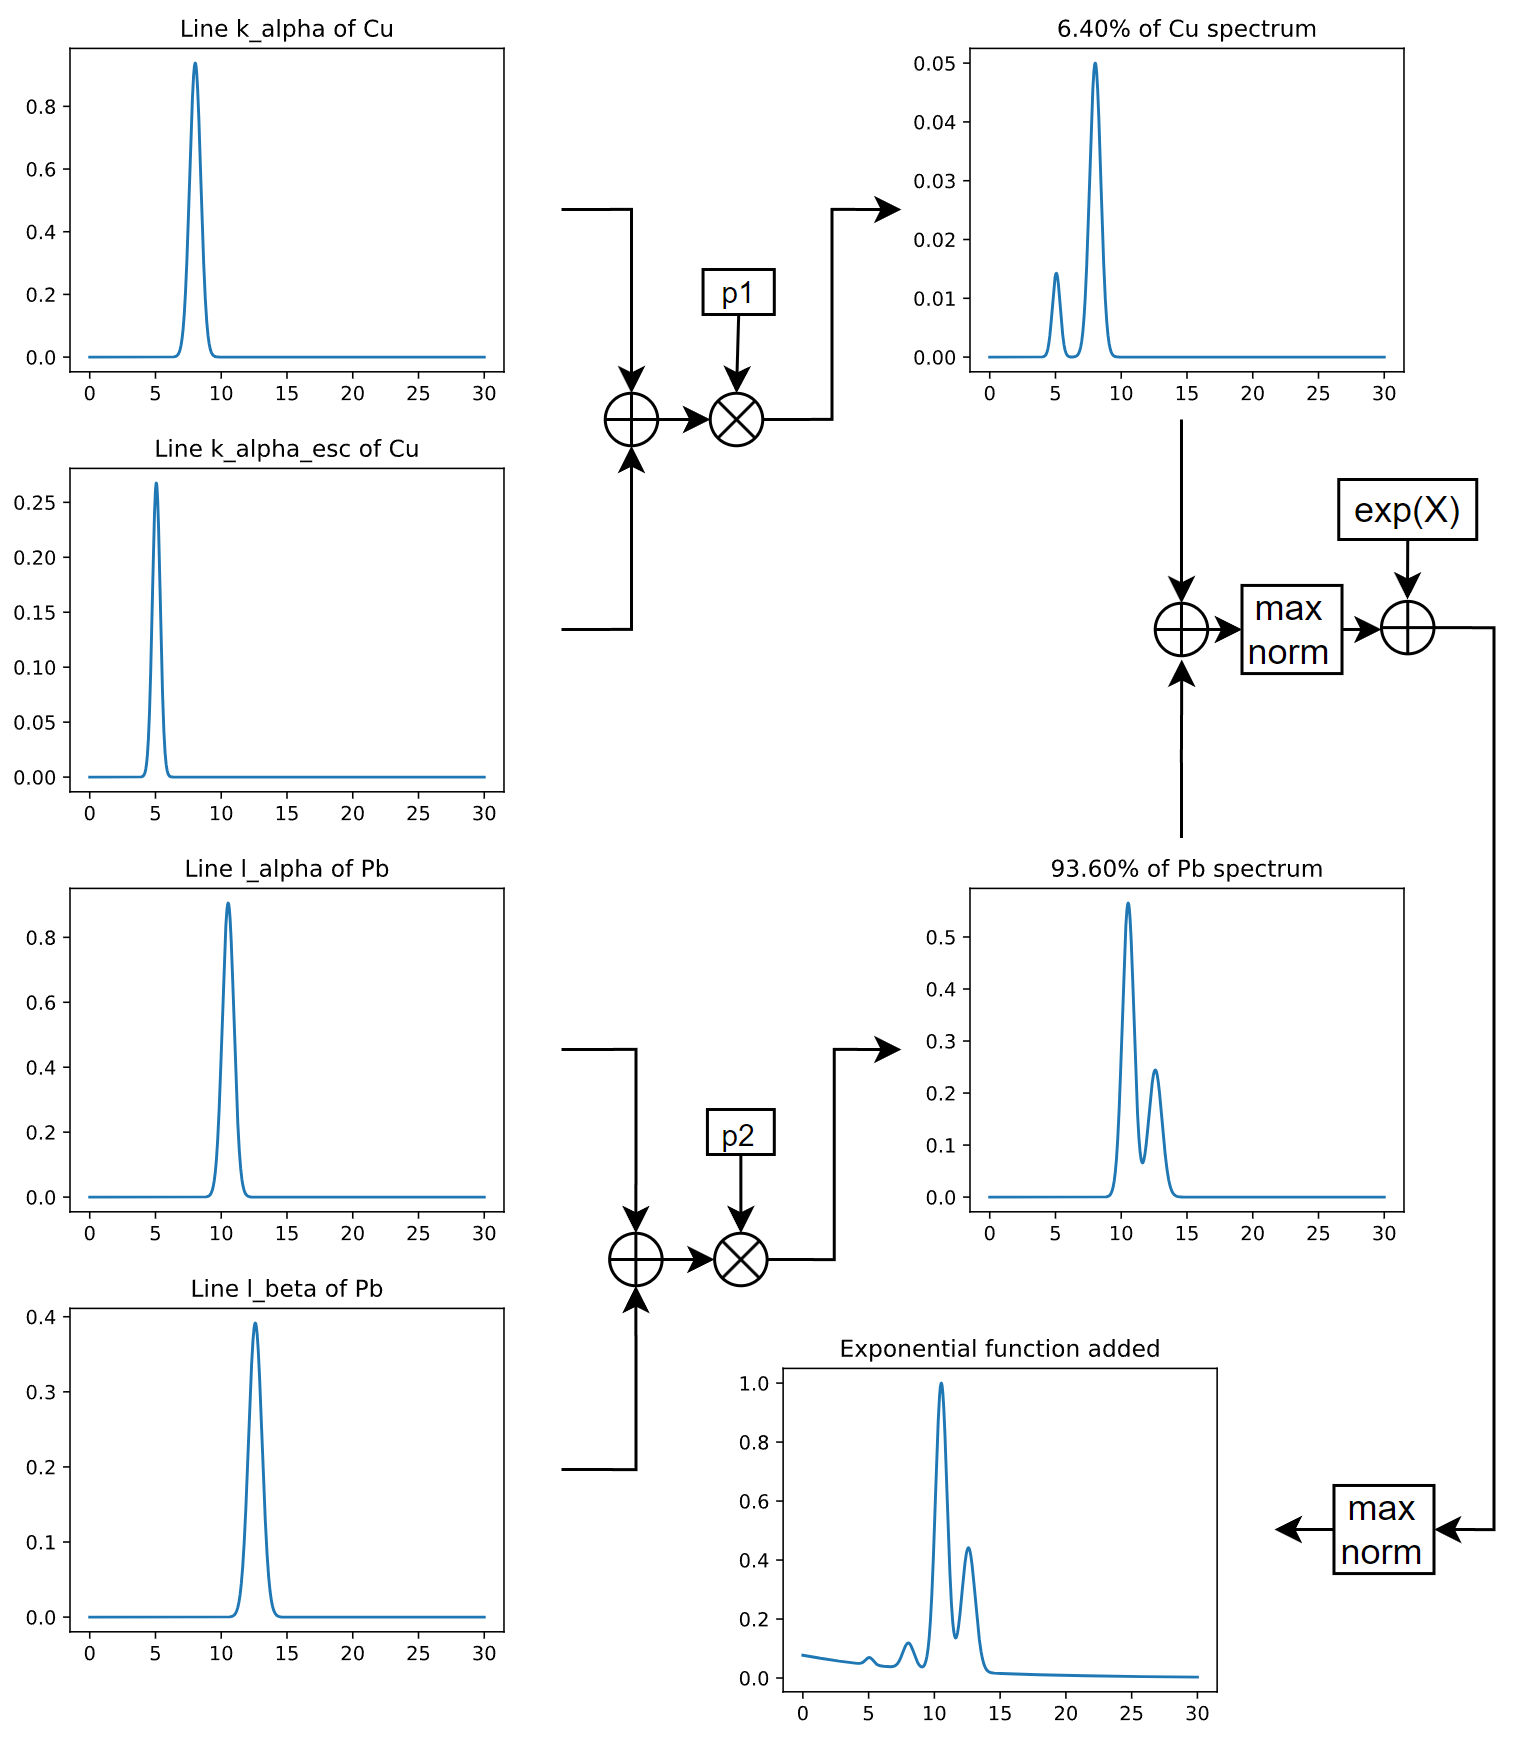
\includegraphics[width=1\textwidth]{img/generation_pipeline.png} 
  \caption{Steps in generation of example training spectrum}
  \label{fig:training_data_generation}
\end{figure}
